\documentclass[sigconf]{acmart}

\usepackage{booktabs} % For formal tables
\usepackage{graphicx}
\usepackage{autobreak}
\usepackage{mytodonotes}
\usepackage{subcaption}
\usepackage{url}
\usepackage[inline]{enumitem}
\usepackage[ruled,vlined]{algorithm2e}
%%%%%%%%%%%%%%%%%%%%%%%%%
\usepackage{cleveref}

% Copyright
%\setcopyright{none}
\setcopyright{acmcopyright}
%\setcopyright{acmlicensed}
%\setcopyright{rightsretained}
%\setcopyright{usgov}
%\setcopyright{usgovmixed}
%\setcopyright{cagov}
%\setcopyright{cagovmixed}


% DOI
\acmDOI{xx.xxx/xxx_x}

% ISBN
\acmISBN{979-8-4007-0629-5/25/03}

%Conference
\acmConference[SAC'25]{ACM SAC Conference}{March 31 –April 4, 2025}{Sicily, Italy}
\acmYear{2025}
\copyrightyear{2025}


\acmArticle{4}
\acmPrice{15.00}

% These commands are optional
%\acmBooktitle{Transactions of the ACM Woodstock conference}
%\editor{Jennifer B. Sartor}
%\editor{Theo D'Hondt}
%\editor{Wolfgang De Meuter}


\begin{document}
\title{Neighbor-Based Decentralized Training Strategies for Multi-Agent Reinforcement Learning}
\titlenote{Produces the permission block, and
  copyright information}
\subtitle{Full Paper}
\subtitlenote{The full version of the author's guide is available as
  \texttt{acmart.pdf} document}
  
\renewcommand{\shorttitle}{SIG Proceedings Paper in LaTeX Format}


%   \institution{University of Bologna}
%   \streetaddress{Via dell'Università, 50}
%   \city{Cesena} 
%   \country{Italy}
% }
% \email{davide.domini@unibo.it}

% \author{Gianluca Aguzzi}
% \affiliation{%
%   \institution{University of Bologna}
%   \streetaddress{Via dell'Università, 50}
%   \city{Cesena} 
%   \country{Italy}\usepackage{algorithm}

% \renewcommand{\shortauthors}{N. Malucelli et al.}

\author{Anonymous Author}
\orcid{1234-5678-9012}
\affiliation{%
  \institution{Anonymous university}
  \country{Anonymous location}
}
% \email{anonymous.author@studio.unibo.it}
\renewcommand{\shortauthors}{A. Author et al.}

\begin{abstract}
Multi-agent deep reinforcement learning (MADRL) is rapidly emerging as a powerful paradigm for training intelligent agents in complex, multi-agent environments.
%
Extending beyond single-agent reinforcement learning, MADRL enables the development  of both collaborative and competitive agents in several domains, like robotics, traffic management, and video games.
%
The most widely adopted training paradigm in MADRL is centralized training with decentralized execution (CTDE), which has demonstrated significant effectiveness. 
%
However, its reliance on a centralized learner necessitates that agents acquire policies offline and subsequently execute them online. 
This inherent constraint motivates the exploration of decentralized training methodologies.
%
While these techniques offer greater flexibility, they tend to have slower convergence and can suffer from instability compared to centralized approaches.
%
Therefore, this paper investigates the effectiveness of various neighbor-based decentralized training strategies based 
  on the well-known Deep-Q Learning algorithm as a viable alternative to centralized training. 
%  
We evaluate experience sharing, k-nearest neighboring averaging, and k-nearest neighboring consensus methods 
  in a cooperative multi-agent environment and compare their performance against centralized training
  and totally decentralized training. 
%  
Our results show that neighbor-based methods can achieve comparable performance to centralized training 
  while offering improved scalability and communication efficiency. 
%
% Finally, we discuss the trade-offs between these methods and provide insights into their applicability 
%   in different scenarios.
\end{abstract}

%
\begin{CCSXML}
<ccs2012>
 <concept>
  <concept_id>10010520.10010553.10010562</concept_id>
  <concept_desc>Computer systems organization~Embedded systems</concept_desc>
  <concept_significance>500</concept_significance>
 </concept>
 <concept>
  <concept_id>10010520.10010575.10010755</concept_id>
  <concept_desc>Computer systems organization~Redundancy</concept_desc>
  <concept_significance>300</concept_sigagentnificance>
 </concept>
 <concept>
  <concept_id>10010520.10010553.10010554</concept_id>
  <concept_desc>Computer systems organization~Robotics</concept_desc>
  <concept_significance>100</concept_significance>
 </concept>
 <concept>
  <concept_id>10003033.10003083.10003095</concept_id>
  <concept_desc>Networks~Network reliability</concept_desc>
  <concept_significance>100</concept_significance>
 </concept>
</ccs2012>  
\end{CCSXML}

\ccsdesc[500]{Computer systems organization~Embedded systems}
\ccsdesc[300]{Computer systems organization~Redundancy}
\ccsdesc{Computer systems organization~Robotics}
\ccsdesc[100]{Networks~Network reliability}


\keywords{Multi-Agent Reinforcement Learning, Decentralized Training, Neighbor-Based Methods, Scalability, Communication Efficiency}
\maketitle

\section{Introduction}
The increasing complexity of real-world systems, from robotic swarms to smart grids, demands intelligent control strategies capable of adapting to dynamic and often unpredictable environments.
%
In this direction, \emph{reinforcement learning} (RL)~\cite{sutton2018reinforcement} has emerged as a powerful paradigm for training agents that interact with their environment and learn optimal policies through trial and error.
%
Moving beyond single-agent settings, \emph{multi-agent reinforcement learning} (MARL)~\cite{bucsoniu2010multi} extends RL to scenarios where multiple agents must collaborate or compete to achieve a common goal.
%
Recent advances in deep learning have further advanced the field, 
enabling the training of complex policies in high-dimensional state and action spaces, 
leading to the emergence of \emph{multi-agent deep reinforcement learning} (MADRL)~\cite{gronauer2022multi}.
%
MADRL has gained significant traction due to its flexibility and capacity to learn diverse behaviors, 
ranging from cooperative~\cite{gupta2017cooperative} to competitive~\cite{tampuu2017multiagent}, 
as demonstrated in various case studies involving video games~\cite{shao2019survey}, robotics~\cite{orr2023multi},
and traffic management~\cite{chu2019multi}. 
%
This paper focuses on the subdomain of \emph{cooperative multi-agent reinforcement learning}, 
a particularly active and impactful area of research within MADRL~\cite{oroojlooy2023review}.

\sloppy
Many prominent approaches in this field employ a centralized training and decentralized execution paradigm
 (e.g.,MAPPO~\cite{yu2022surprising}, MADDPG~\cite{DBLP:conf/nips/LoweWTHAM17}, QMIX~\cite{DBLP:conf/icml/RashidSWFFW18}, QTRAN~\cite{DBLP:conf/icml/SonKKHY19}), 
 where a centralized learner trains distributed policies that are subsequently executed independently. 
%
While facilitating decentralized runtime operation and avoiding single points of failure, 
 this approach typically entails an offline learning phase (using simulators and centralized computation) 
 followed by online execution with no further learning. 
 This inherent limitation hinders adaptation to changing environments or tasks at runtime, like those encountered in real-world robotics applications.  
% 
While fully independent learners~\cite{abed2016comparison} offer a potential solution for online learning,
 they often underperform centralized counterparts due to instability in training and a lack of differentiation between agents and their interactions with the environment. 
%
Inspired by many real-world multi-agent systems in which 
 agents only interact with a limited subset of the overall system (also called \emph{networked agents})--as exemplified by limited sensing ranges in swarm robotics or localized interactions--in this paper proposes and formalizes a family of distributed learning methodologies based on neighborhood information.
This approach aims to: 
i) incorporate richer information compared to independent learners, and
ii) facilitate the emergence of collective behaviors through local interactions between networked agents.
Specifically, we investigate three distinct neighboring-based training strategies encompassing both neural network-based approaches 
(e.g., neighboring averaging and consensus) 
and experience-based methods inspired by centralized experience sharing~\cite{DBLP:conf/nips/ChristianosSA20}. 
We demonstrate the effectiveness of these strategies in comparison to both centralized and fully distributed approaches, 
highlighting how neighborhood-based policies offer a compelling compromise between these two extremes.

The remainder of this paper is structured as follows.
\Cref{sec:background} provides an overview of multi-agent reinforcement learning,
highlighting the key challenges and training paradigms.
\Cref{sec:neighboring} introduces the proposed neighboring-based training strategies,
detailing their implementation and operation.
\Cref{sec:experiments} presents the experimental setup and evaluation metrics.
\Cref{sec:results} discusses the results of the experiments,
comparing the performance of the neighboring-based methods against centralized training.
Finally, \Cref{sec:conclusion} concludes the paper,
summarizing the key findings and outlining potential future research directions.

\section{Background and Motivation}\label{sec:background}
Multi-agent reinforcement learning (MARL) involves a group of \emph{agents} interacting with a shared \emph{environment}. 
%
At each timestep, agents receive \emph{observations} and select \emph{actions} according to their individual \emph{policies} (mappings from observations to actions). 
%
These individual actions combine to form a \emph{joint action}, which influences the environment's transition to a new state. 
%
Each agent then receives a scalar \emph{reward} signal, typically a function of the global state and joint action. 
%
The goal of each agent is to maximize its cumulative reward. 
%
Environments can be \emph{partially observable}, meaning agents may not have access to the full global state, only receiving local observations through their respective \emph{observation functions}.
 
%In this paper, we focus on cooperative MARL scenarios, 
%where agents must collaborate to achieve a common goal.
%In the following, we provide an overview of the key concepts in MARL, 
%including the formalization of the problem, the deep Q-learning algorithm, and the training paradigms used in the literature.
\subsection{Formalization}
Since MARL is a broad field, it is essential to provide a formalization to guide the discussion.
In this paper, we consider partially observable networked markov decision process (PONMDP)~\cite{DBLP:journals/tac/AdlakhaLG12} as a tuple $(\mathcal{G}, \mathcal{S}, \mathcal{A}, \mathcal{O}, \mathcal{P}, \mathcal{R}, \gamma)$, where

\begin{itemize}
  \item $\mathcal{G} = (N, E)$ is a communication graph, where $N$ is the set of $n$ agents and $E \subseteq N \times N$ represents the communication links between agents. 
  Time-varying graphs $\mathcal{G}_t = (N, E_t)$ can be used to represent communication evolving over time $t$.
  \item $\mathcal{S}$ is the global state space.
  \item $\mathcal{A} = \mathcal{A}^1 \times \dots \times \mathcal{A}^n$ is the joint action space, where $\mathcal{A}^i$ is the action space of agent $i$.
  \item $\mathcal{O} = \mathcal{O}^1 \times \dots \times \mathcal{O}^n$ is the joint observation space, where $\mathcal{O}^i$ is the observation space for agent $i$.
  \item $\mathcal{P}: \mathcal{S} \times \mathcal{A} \times \mathcal{S} \to [0, 1]$ is the state transition function, describing the probability of transitioning to a new state $s' \in \mathcal{S}$ given the current state $s \in \mathcal{S}$ and joint action $a \in \mathcal{A}$.
  \item $\mathcal{R} = {\mathcal{R}^i}_{i \in N}$, where $\mathcal{R}^i: \mathcal{S} \times \mathcal{A} \to \mathbb{R}$ is the reward function for agent $i$.
  \item $\gamma \in [0, 1]$ is the discount factor.
\end{itemize}
Each agent $i$ at time $t$ receives an observation $o^i_t \in \mathcal{O}^i$, 
takes an action $a^i_t \in \mathcal{A}^i$ based on its local policy $\pi^i: \mathcal{O}^i \times \mathcal{A}^i \to [0,1]$, and receives a reward $r^i_{t+1} = \mathcal{R}^i(s_t, a_t)$. 
%
The global state evolves according to $\mathcal{P}$. 
Agents can exchange information with their neighbors in $\mathcal{G}$ 
(or $\mathcal{G}t$ if the graph is time-varying). 
%
The objective is typically to maximize the expected discounted sum of rewards $\sum{t=0}^{\infty} \gamma^t r^i_t$ for each agent $i$, 
or some global reward function like the average reward over all agents in case of cooperative scenarios.
%Formally, it can be defined as:
%\[ J(\{\pi^i\}) = \lim_{T \to \infty} \mathbb{E} \left[ \frac{1}{T} \sum_{t=0}^{T-1} \frac{1}{N} \sum_{i \in \mathcal{N}} R^i(s_t, a_t) \right] \]
Agents typically use other function to estimate the value of taking an action in a given state, such as the action-value function (also known as \emph{Q-value}). 
The latter represents the expected cumulative discounted reward the agent will receive by taking action $a \in \mathcal{A}$ in state $s \in \mathcal{S}$ and then following its policy $\pi^i$:

\[ Q^i(s, a) = \mathbb{E}_{\pi^i} \left[ \sum_{t=0}^{\infty} \gamma^t r^i_{t+1} | s_0 = s, a_0 = a \right] \]

%Similar to the individual reward function, a global average reward function can be defined as $\bar{\mathcal{R}}(s, a) = \frac{1}{n} \sum_{i=1}^n \mathcal{R}^i(s,a)$, leading to a global average Q-value:

%\[ \bar{Q}(s, a) = \mathbb{E}_{\pi} \left[ \sum_{t=0}^{\infty} \gamma^t \bar{\mathcal{R}}(s_t, a_t) | s_0 = s, a_0 = a \right] \]

%where $\pi = \{\pi^i\}_{i \in N}$ represents the joint policy. 
%The goal in collaborative MARL is often to find a joint policy that maximizes this global average Q-value or a similar global objective.
Several algorithms aim to find the \emph{optimal} Q-value function, which maximizes the expected cumulative reward. 
%
One of the most popular among these is the Deep Q-learning algorithm.
\subsubsection{Deep Q-Learning Formalization}
Deep Q-learning~\cite{DBLP:conf/l4dc/FanWXY20} utilizes a deep neural network, 
often referred to as a Q-network, to approximate the action-value function $Q(s, a)$. 
This network takes the state $s$ as input and outputs a vector of Q-values, one for each possible action $a \in \mathcal{A}$.  
The optimal action-value function, denoted $Q^*(s, a)$, satisfies the Bellman optimality equation:

\[ Q^*(s, a) = \mathbb{E}_{s' \sim \mathcal{P}} \left[ r + \gamma \max_{a'} Q^*(s', a') | s, a \right] \]

where $\mathcal{P}$ is the state transition probability distribution.  
Deep Q-learning aims to train the Q-network to approximate $Q^*(s, a)$ by minimizing the loss function:

\[ \mathcal{L}(\theta) = \mathbb{E}_{(s, a, r, s') \sim \mathcal{D}} \left[ \left( r + \gamma \max_{a'} Q(s', a'; \theta^-) - Q(s, a; \theta) \right)^2 \right] \]

where $\theta$ are the parameters of the Q-network, $\theta^-$ are the parameters of a target Q-network (used for stability), 
and $\mathcal{D}$ is the experience replay buffer, a collection of past experiences $(s, a, r, s')$.
%
In the multi-agent setting, each agent $i$ has its own Q-network $Q^i(o^i, a^i; \theta^i)$ that takes its local observation $o^i$ as input.  
For centralized training, the global state $s$ can be used as input. 
The specific form of the multi-agent Q-function and the update rules depend on the chosen MARL algorithm (e.g., distributed Deep Q-learning~\cite{ong2015distributed}, value decomposition methods~\cite{DBLP:conf/icml/SonKKHY19}).  
%For example, in independent Deep Q-learning--more details in \Cref{sec:sota}--each agent updates its Q-network independently using its local reward $r^i$:
%\begin{equation}
%  \resizebox{\linewidth}{!}{$
%  \mathcal{L}^i(\theta^i) = \mathbb{E}_{(o^i, a^i, r^i, o'^i) \sim \mathcal{D}^i} \left[ \left( r^i + \gamma \max_{a'^i} Q^i(o'^i, a'^i; \theta^{i-}) - Q^i(o^i, a^i; \theta^i) \right)^2 \right]
%  $}
%  \end{equation}
%\subsection{Key Concepts}

\subsection{Learning Schemes}
\begin{figure}
  \centering
  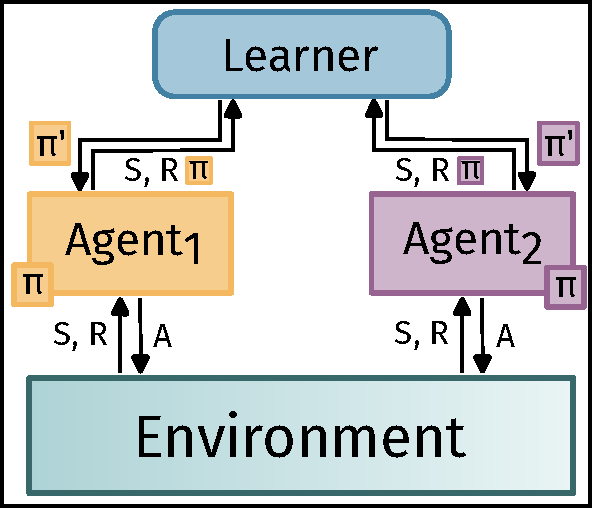
\includegraphics[width=0.7\linewidth]{figures/CTDE.pdf}
  \vskip 1 mm
  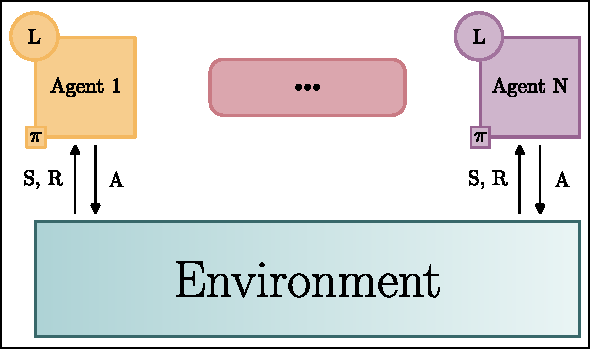
\includegraphics[width=0.7\linewidth]{figures/DTDE.pdf}
  \caption{Graphical representation of centralized training with decentralized execution (left) and decentralized training with decentralized execution (rigth) in multi-agent reinforcement learning.}
  \label{fig:learning_paradigms}
\end{figure}
Multi-agent learning can be categorized based on the training scheme and the information accessibility for agents. 
Two prominent paradigms are centralized training with decentralized execution (CTDE) and decentralized training with decentralized execution (DTDE)---see \Cref{fig:learning_paradigms}.

\paragraph{Centralized Training with Decentralized Execution (CTDE)}
In CTDE, a central learner trains all agents, 
but execution of the learned policy is decentralized. 
This process typically involves two phases:
\begin{enumerate}
  \item \textit{Offline training:} Agents interact with a simulator or environment, gathering experience data used to update the central learner's policy.
  \item \textit{Online execution:} Agents deploy the learned policy in the environment without further learning.
\end{enumerate}
This approach offers several benefits.  
Leveraging a centralized dataset allows for efficient learning, 
potentially exploiting global information, 
which is crucial in cooperative scenarios requiring coordinated actions. 
Furthermore, decentralized execution allows agents to act independently after training.
%
However, CTDE has limitations. 
Scalability can become problematic with a large number of agents. 
The reliance on a central learner hinders adaptation to dynamic environments or tasks during runtime.
\sloppy
\paragraph{Decentralized Training with Decentralized Execution (DTDE)}
DTDE eliminates the central learner; each agent learns independently from its own experiences.
Inter-agent cooperation and communication can be incorporated during both training and execution. 
Unlike CTDE, training and execution phases are not necessarily separate---simultaneous learning and execution allow for adaptation to 
changing environments or tasks at runtime.
%
Key advantages of DTDE include scalability with the number of agents and adaptability to dynamic environments.
%
However, DTDE also presents several challenges to overcome, like: 
i) convergence time is often longer compared to centralized training. 
ii) The lack of central coordination can lead to instability and difficulties in differentiating agents and their environmental interactions; and 
iii) online learning in DTDE can introduce non-stationarity if agents do not account for other agents' evolving policies during training, 
as the environment effectively changes from each agent's perspective.

\subsection{State of the Art}\label{sec:sota}
MARL is a longstanding research area with a rich literature, starting 
from seminal works like~\cite{tan1993multi} and~\cite{busoniu2008comprehensive} to more recent contributions like~\cite{gronauer2022multi} and~\cite{canese2021multi}.
%
In the following, we briefly discuss some of the most relevant approaches in the field, which lead to the motivation for our work.
\subsubsection{Independent Learners}
In independent learners, each agent learns its policy independently, disregarding the actions and policies of other agents. 
This straightforward approach, among the earliest explored in MARL, often relies on variants of Q-learning. 
%
Several algorithms have attempted to address these coordination challenges within the independent learner paradigm. 
Basic decentralized Q-learning~\cite{tan1993multi} allows each agent to learn its Q-values independently but often converges to suboptimal joint policies due to a lack of coordination. 
Subsequent work introduced heuristic-based extensions to improve coordination.
Approaches like distributed Q-learning~\cite{lauer2000algorithm} incorporate optimism in Q-value updates and equilibrium selection mechanisms to mitigate the convergence to shadowed equilibria (i.e., equilibria that are unstable due to the independent learning processes). 
Instead, algorithms such as hysteretic Q-learning~\cite{matignon2007hysteretic}, lenient Q-Learning~\cite{bloembergen2010lenient} and win-or-learn fast policy hill climbing~\cite{bowling2002multiagent} employ adaptive learning rates to address the issue of alternating exploration between agents, improving robustness and convergence.
%
Empirical comparisons of these algorithms highlight the trade-offs in performance across various MARL tasks and coordination challenges~\cite{matignon2012independent}. 
While initially developed for tabular settings, some of these methods, like hysteretic Q-learning~\cite{palmer2017lenient} and lenient Q-learning, have been extended to deep reinforcement learning settings. 
However, these independent approaches, even with deep learning, often exhibit instability and slow convergence in complex environments and fundamentally lack explicit mechanisms for inter-agent coordination. 
%Consequently, more sophisticated MARL algorithms have been developed that explicitly account for the interactions and policies of other agents to facilitate more effective coordination.
\subsubsection{Neighboring-Based Methods}
Neighboring-based methods in MARL address the scalability and communication overhead challenges of fully centralized approaches by restricting agent interactions to a local neighborhood. 
This introduces agents communication and coordination with a limited set of neighbors, reducing the complexity of full joint action and policy learning.
%
One prominent category within neighboring-based methods is \emph{consensus-based} algorithms. 
These algorithms aim to reach a consensus among agents on shared values or policies through local information exchange. 
Early work like QD-learning~\cite{kar2012qd} extends Q-learning with a consensus update term, 
enabling agents to converge towards optimal Q-values despite only receiving local rewards.
%  
Recent advances in consensus-based MARL leverage deep learning and actor-critic architectures, 
combining local policy updates with consensus updates on critic parameters or gradients, 
as seen in the recent works~\cite{7434032,pennesi2010distributed,zhang2018fully,DBLP:journals/jmlr/CiosekW20}.

These algorithms often exhibit improved scalability and communication efficiency compared to fully centralized methods, 
but still need lack in capturing the global structure of the environment and the interactions between agents.
\subsubsection{Centralized Training Methods} CTDE is a prominent paradigm in MARL~\cite{ning2024survey}, 
leveraging centralized information during training to learn decentralized policies for execution. 
This approach addresses the challenges of partial observability and non-stationarity while maintaining the scalability of decentralized execution. % 
Actor-critic methods are well-suited for the CTDE paradigm, 
where a centralized critic provides feedback to decentralized actors~\cite{DBLP:conf/icml/RashidSWFFW18,DBLP:journals/corr/SunehagLGCZJLSL17,yu2022surprising,DBLP:conf/nips/LoweWTHAM17}. 
% 
The most influential algorithms in this area are the one called \emph{policy-based} methods (i.e., the ones that learn a policy directly).
%
Multi-agent deep deterministic policy Gradient (MADDPG)~\cite{DBLP:conf/nips/LoweWTHAM17} employs a centralized critic that has access to the states and actions of all agents, providing more informative feedback for policy updates. 
Each agent then learns a deterministic policy based on its local observations. % 
Building on the actor-critic framework, Multi-Agent Proximal Policy Optimization (MAPPO)~\cite{yu2022surprising} extends the centralized critic concept to the policy optimization setting. 
MAPPO leverages a centralized critic to estimate advantage functions for policy updates, while individual agents learn stochastic policies. 
%This approach has shown promising results in various cooperative and competitive MARL tasks, exhibiting improved sample efficiency and robustness compared to MADDPG. % 
Another class of algorithms, called \emph{value-based} methods, learn a value function that estimates the expected return for each agent.
%
Value Decomposition Networks (VDN)~\cite{DBLP:journals/corr/SunehagLGCZJLSL17} and QMIX~\cite{DBLP:conf/icml/RashidSWFFW18} are representative algorithms in this category. 
VDN factorizes the joint Q-function into a sum of individual agent Q-functions, 
simplifying the learning process. 
QMIX improves upon VDN by learning a monotonic mixing function that combines individual Q-values, 
allowing for more complex representations of joint action values. % 
%
Another approach to address the scalability challenge in MARL is \emph{mean field reinforcement learning}, i.e., 
the one that models the interaction between agents through a mean field, simplifying the multi-agent problem into a single-agent problem against an average opponent.
%
In this context, mean field q-learning (Mean-Q)~\cite{DBLP:conf/icml/YangLLZZW18} has been proposed.
This approach scales well to large numbers of agents and has been successful in various applications. 
% 
There are also modern solution which leverages collective abstraction to reduce the complexity of the problem, such as the one proposed in field-informed reinforcement learning~\cite{DBLP:conf/acsos/AguzziVE23}.
\subsection{Motivation}
MADRL faces a critical challenge in balancing scalability and performance.  
Centralized training methods, while effective, often suffer from computational bottlenecks and difficulties scaling to large numbers of agents. 
While distributed training approaches offer improved scalability, 
they frequently assume independent learners, 
neglecting crucial inter-agent coordination and leading to suboptimal global performance.  
%
Neighbor-based methods have shown promise in simpler, 
tabular settings by enabling localized coordination,
but their integration with deep reinforcement learning remains largely unexplored. 
This work bridges this gap by introducing a novel approach that combines the power of deep learning with the scalability of neighbor-based communication.  
Our method aims to achieve both efficient decentralized learning and effective coordination, 
enabling online adaptation and robust performance in complex multi-agent environments.

\section{Neighboring-Based Distributed Learning Strategies}\label{sec:neighboring}
This section introduces three neighboring-based distributed learning strategies for multi-agent reinforcement learning.
These strategies leverage local interactions between agents to improve learning efficiency and coordination.
For this investigation, we focus on deep Q-learning as the underlying learning algorithm,
and we consider the following strategies: k-nearest neighbor averaging, k-nearest neighbor consensus, and experience sharing.

\paragraph{K-Nearest Neighbor Definition}
The proposed strategies rely on the concept of k-nearest neighbors.
Formally, consider a \emph{weighted} communication graph $\mathcal{G} = (N, E, W)$, where $N$ is the set of agents, where $W: E \rightarrow \mathbb{R}^+$ is a weight function assigning a positive weight to each edge.  
Let $d(i,j)$ denote the shortest path length between agents $i$ and $j$ in the weighted graph $\mathcal{G}$. 
This can be calculated, for instance, using Dijkstra's algorithm. 
The length of a path is the sum of the weights of the edges along the path. 
If no path exists between $i$ and $j$, we set $d(i,j) = \infty$.
%
Then, the set of $k$-nearest neighbors of agent $i$ is defined as:
$$ \mathcal{N}_k(i) = { j \in N \setminus {i} \mid \text{rank}(d(i,j)) \leq k } $$
where $\text{rank}(d(i,j))$ denotes the rank of the distance $d(i,j)$ among all distances from agent $i$ to other agents in $N \setminus {i}$, sorted in ascending order (e..g, $\text{rank}(d(i,j)) = 1$ for the smallest distance).
Ties can be broken arbitrarily.

\paragraph{K-Nearest Neighbor Averaging}
\sloppy
This approach averages an agent's Q-values with those of its nearest neighbors. 
Each agent maintains a local Q-network and shares its Q-values with its neighbors. 
The neighbors average the received Q-values and use the result to update their own Q-networks. 
This leverages the collective knowledge of neighboring agents to improve learning.
%
Formally, giving $\theta^t_i, i \in N$ the parameters of the Q-networks of the agent $i$ at the time $t$,
the update rule for agent $i$ at time $t+1$ is:
\begin{equation}
  \theta^{t+1}_i = \theta^t_i + \alpha \sum_{j \in \mathcal{N}_k(i)} \frac{1}{k} \theta^t_j
\end{equation}

\paragraph{K-Nearest Neighbor Consensus}
In case of homogeneous agents (i.e., when all agents have the same action and observation space),
the goal of learning is to find a common policy that all agents can follow.
This approach is typically used in large-scale systems where agents are identical and need to reach a consensus---see~\cite{DBLP:conf/eusipco/BaldazoPZ19}.
%
In this case, instead of forcing a common policy, we can let agents learn independently and then select the best-performing agent as the reference for the others, leading eventually to a consensus on the best same policy.
%
In this way, each agent $i$ continue to learn independently, but at each iteration, it updates its Q-network using the Q-values of the best-performing agent in its neighborhood.
%
The best performing agent is selected based on the average reward it has received in the last $n$ episodes.
Formally, the update rule for agent $i$ at time $t+1$ is:
\begin{equation}
  \theta^{t+1}_i \leftarrow \theta^t_{\text{best}}
\end{equation}
where $\theta^t_{\text{best}}$ is the Q-network of the best-performing agent in the neighborhood $\mathcal{N}_k(i)$ at time $t$.

\paragraph{Experience Sharing}
Experience sharing is a simple yet effective method for distributed learning.
This approach is typically used in centralized training to improve sample efficiency and learning stability~\cite{marl-book}.
In our distributed setting, each agent maintains its own experience replay buffer, 
but it also shares a fraction of its experiences with its neighbors.
This allows agents to learn from each other's experiences, 
potentially accelerating learning and improving coordination because agents can learn from each other's mistakes and successes.
%
Formally, the reply buffer of agent $i$ at time $t$ is $\mathcal{D}^t_i = \{(o^i, a^i, r^i, o'^i)\}$.
At each iteration, agent $i$ shares a fraction $\beta$ of its experiences with its neighbors in $\mathcal{N}_k(i)$.
The update rule for agent $i$ at time $t+1$ is:
\begin{equation}
  \mathcal{D}^{t+1}_i = \mathcal{D}^t_i \cup \bigcup_{j \in \mathcal{N}_k(i)} \beta \mathcal{D}^t_j
\end{equation}
\paragraph{Neighboring-Based Training with Deep Q-Learning}
The neighboring-based training strategies can be integrated with deep Q-learning to enable distributed learning in multi-agent settings.
%
The algorithm follow the same structure as the deep Q-learning algorithm, 
but with the addition of the neighboring-based intereactions.
%
This may happen with a different frequency for each strategy, 
depending on the communication overhead and the desired level of coordination.

In \Cref{alg:neighbor_dqn} we provide a detailed description of the integration of the neighboring-based strategies with deep Q-learning.
\begin{algorithm}
  \caption{Neighboring-Based Deep Q-Learning}
  \label{alg:neighbor_dqn}
  \ForEach{agent $i \in N$}{
      Initialize Q-network $Q^i(o^i, a^i; \theta^i)$ and target network $Q^{i-}(o^i, a^i; \theta^{i-})$\\
      Initialize replay buffer $\mathcal{D}^i$
  }
  \For{episode = 1 to M}{
      \ForEach{agent $i \in N$}{
          Initialize initial observation $o_0^i$
      }
      \For{t = 0 to T}{
          \ForEach{agent $i \in N$}{
              Select action $a_t^i$ based on $\epsilon$-greedy policy using $Q^i(o_t^i, a^i; \theta^i)$\\
              Execute action $a_t^i$ and observe reward $r_{t+1}^i$ and next observation $o_{t+1}^i$\\
              Store $(o_t^i, a_t^i, r_{t+1}^i, o_{t+1}^i)$ in $\mathcal{D}^i$\\
              Sample a mini-batch from $\mathcal{D}^i$\\
              Calculate target values using chosen neighboring strategy (see below)\\
              Update $\theta^i$ by minimizing the TD error\\
              Every C steps, update target network $\theta^{i-} \leftarrow \theta^i$\\
              \textbf{
              Every S steps, perform neighboring strategy}
          }
      }
  }
\end{algorithm}
\section{Evaluation}\label{sec:experiments}
This section presents the experimental setup and evaluation metrics used to assess the performance of the proposed neighboring-based training strategies.
All the experiments and data produced are reproducible and publicly available\footnote{\url{https://anonymous.4open.science/r/experiments-2024-SAC-marl-neighbouring-strategies-4B8F}}.
\subsection{Simulated environment}
The proposed multi-agent environment is a variant of the ``gather the items'' scenario, designed to study the impact of neighborhood strategies. 
It consists of a 2D Euclidean space populated by $A$ agents and $T$ targets, 
initially placed at random locations.
%
The objective is for the agents to collectively capture all targets, 
at which point the environment episode terminates successfully.  
A maximum time limit of $T_{max} = 300$ time steps is enforced to prevent indefinite episodes.

At each time step $t$, each agent $a$ receives an observation $o_a^t$ composed of the following elements:
\begin{itemize}
  \item \emph{Neighborhood perception}:  Agent $a$ perceives the relative positions (distance and direction) of its $A_v$ nearest neighboring agents. 
  This information is represented as a set $\mathcal{V}_a^t = \{(d_{aj}^t, \theta_{aj}^t) | j \in \text{Nearest } A_v \text{ agents}\}$, 
  where $d_{aj}^t$ is the Euclidean distance between agent $a$ and agent $j$ at time $t$, and $\theta_{aj}^t$ is the angle between the vector pointing from agent $a$ to agent $j$ and a fixed reference axis.
  \item \emph{Target perception}: Agent $a$ perceives the relative positions (distance and direction) of its $T_v$ nearest targets. 
  This is represented as a set $\mathcal{T}_a^t = \{(d_{ak}^t, \theta_{ak}^t) | k \in \text{Nearest } T_v \text{ targets}\}$, with $d_{ak}^t$ and $\theta_{ak}^t$ defined analogously to the neighborhood perception.
  \item \emph{Memory}: Agent $a$ maintains a memory $\mathcal{H}_a^t$ of past perceptions, storing the neighborhood and target perceptions from the previous $H_t$ time steps. Formally, $\mathcal{H}_a^t = \{\mathcal{N}_a^{t-\tau}, \mathcal{T}_a^{t-\tau} | \tau = 1, \dots, H_t\}$. 
  This can be represented as a tensor of shape $(H_t, A_v + T_v, 2)$, where the last dimension represents the relative distance and angle for each perceived agent or target.
\end{itemize}
The complete observation $o_a^t$ at time $t$ for agent $a$ is thus given by $o_a^t = (\mathcal{N}_a^t, \mathcal{T}_a^t, \mathcal{H}_a^t)$.

Communication between agents is restricted to a neighborhood $\mathcal{C}_a^t \subseteq \mathcal{N}_a^t$ 
and depends on a communication graph $\mathcal{G}$.
%
This communication enables the exchange of information such as Q-values or experiences 
using on of the neighboring-based strategies discussed in \Cref{sec:neighboring}.
%
The action space for each agent is discrete, consisting of eight possible movements corresponding to the cardinal and diagonal directions on a grid.

This environment provides a challenging coordination problem, 
requiring agents to learn individual target-seeking behaviors and collaborative strategies 
to minimize retrieval time. 
%
It serves as a suitable testbed for evaluating the effectiveness 
of neighbor-based decentralized training approaches.
\subsubsection{Reward function}
In the proposed environment, we design a reward function that both consider the individual performance of each agent (e.g., avoid collision) and the global performance of the team (e.g., collect items in the shortest time possible).
In the following, we describe the components of the reward function:
\paragraph{Collisions} Agents are penalized when their action area intersect. This penalty is proportional to the number of agents involved in a collision:
  \[ \psi = \begin{cases}
    0 & \text{if no intersections} \\
    -2 \cdot |I_a| & \text{otherwise}
  \end{cases} \]
where $I_a$ is the set of agents with intersecting action area.

\paragraph{Time step} Agents are penalized at each time step by a constant value $\sigma$ defined as
    an hyperparameter, to encourage them to complete the task as quickly as possible.
    \[ \zeta = - \sigma \]
 
\paragraph{Moving towards items} Each agent $a$ is rewarded if it moves towards one of the visible target items, discouraging agents from wandering aimlessly.
    \[ \xi = (max_{i \in V_{items}} d(p_a^{t+1}, p_i^{t+1}) - d(p_a^{t}, p_i^{t})) \cdot \delta\]
    Where $p_a^t$ is the position of the agent $a$ at time t (similarly for $p_i^{t}$ regarding items),
    $\delta$ is a scalar hyperparameter used to tune the importance of this component and
    $V_{items}$ is the set of visible items.
\paragraph{Moving away from agents} Each agent $a_i$ is rewarded if it increases the distance from its neighbors ($N_{a_i}$). This strategy encourages agents to avoid clustering and explore the environment more effectively.
    \[ \chi = \frac{1}{2|N_{a_i}|} \cdot \sum_{a_j \in N_{a_i}} d(p_{a_i}^{t+1}, p_{a_j}^{t+1}) - d(p_{a_i}^{t}, p_{a_j}^{t}) \]

\paragraph{Collecting items} Each agent is rewarded for any collected visible items ($C_i$ is the set of collected items), 
    whether the item was collected by  the agent itself or by another agent, this strategy encourages agents 
    to develop cooperative behaviors.
    \[ \rho = 100 \cdot |C_i| \]

\paragraph{Final reward} The final reward is computed as the sum of all the subcomponents:
  \[ R = \psi + \zeta + \xi + \chi + \rho \]
  
\subsection{Experimental setup}
The described environment was implemented using the \emph{Gymnasium} framework~\cite{DBLP:journals/corr/abs-2407-17032}.
Moreover, we employed the following libraries to implement the learning algorithms namely: \emph{Ray}~\cite{DBLP:conf/osdi/MoritzNWTLLEYPJ18} 
  (in particular, its module \emph{RLlib}~\cite{DBLP:conf/icml/LiangLNMFGGJS18}),
  and \emph{PyTorch}~\cite{DBLP:conf/nips/PaszkeGMLBCKLGA19}.

We ran a total of $42$ training experiments, 
namely: $6$ different methods %% TODO check how many ex are discussed
  (centralized, distributed and the three neighbor-based strategies discussed).
Each method was evaluated across 10 distinct random seeds to enhance the statistical robustness of the observed results.
%
Each experiment consisted of $50$ training episodes. 
%
Furthermore, we ran $15$ evaluation experiments, namely: $5$ different methods and for each method 
  we varied the number of agents ($8$, $16$ and $32$) to assess the metrics under various conditions.
  In this case, for each experiment we ran $100$ evaluation episodes.

\subsection{Learning algorithm}
In our experiments, we employed the well-known \emph{Deep Q-Learning} (DQN) algorithm implemented in RLlib.
%
We set the discount factor $\gamma$ to $0.95$, this parameter controls how much future rewards are 
  considered in the decision-making process.
%
A value slightly below $1$ encourages the agent to prioritize immediate rewards while still accounting 
  for long-term benefits, striking a balance between short-term and long-term planning.
%
We chose a learning rate of $0.001$ to control the speed at which the Q-network's weights are updated.
%
This relatively low learning rate ensures stable learning, preventing large updates that could destabilize 
  the training process, specially in complex environments with multiple interacting agents.
%
For the training batch size, we used a value of $32$, which balances computational efficiency and the diversity 
  of experiences in each update. 
%
A smaller batch size could lead to noisier updates, while a larger one might slow down training without
  significantly improving performance.
%
%Additionally, we enabled two key features of the DQN algorithm, namely:
%  \begin{enumerate*}[label=(\roman*)]
%    \item \emph{Double Q-Learning}, to mitigate the overestimation bias that traditional Q-Learning algorithms are prone to. 
%      This is particularly important in multi-agent settings, where overestimation can lead to suboptimal policies due to 
%      the complex interactions between agents ; and
%    \item \emph{Dueling Q-Learning}, which separates the estimation of the state value from the state-dependent action advantages, 
%      enabling the agent to better distinguish between the value of being in a given state and the value of choosing 
%      specific actions within that state.
%  \end{enumerate*} 

\subsection{Evaluation metrics} 
In our experiments, we employed two metrics to evaluate the performance of the learning
  agents and monitor the quality of the training process, namely: 
  \begin{enumerate*}[label=(\roman*)]
    \item \emph{Mean Episode Reward} ($R_{mean}$); and
    \item \emph{Mean Episode Length} ($L_{mean}$).
  \end{enumerate*} 
%
$R_{mean}$ measures the average cumulative reward the agent obtains during each episode, 
  serving as a direct indicator of how well each agent is performing in achieving its task.
%
Formally, for $N$ episodes, the mean reward $R_{mean}$ is computed as:
  \[ R_{mean} = \frac{1}{N} \sum_{i=1}^{N} R_i \]
  where $R_i$ is the total reward obtained by all agents in the $i$-th episode. 
  Formally, for a certain episode $i$, composed of $n$ agents, last $T$ time steps, the total reward $R_i$ is calculated as:
  \[ R_i = \sum_{t=0}^{T} \sum_{j=1}^{n} r^j_t \]
  where $r^j_t$ is the reward obtained by agent $j$ at time step $t$.


On the other hand, the $L_{mean}$ represents the average number of time steps needed to reaching the terminal state, i.e., no more items to collect. 
%
It provides insights into the agent's efficiency in completing tasks, especially in environments 
  where shorter episodes indicate better performance.
%
The mean episode length $L_{mean}$ is calculated as:
  \[ L_{mean} = \frac{1}{N} \sum_{i=1}^{N} L_i \]
  where $L_i$ is length of $i$-th episode.


% \begin{figure}
%   \centering
%   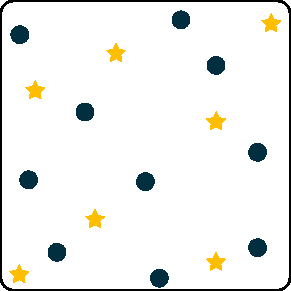
\includegraphics[width=0.7\linewidth]{figures/env.pdf}
%   \caption{Graphical representation of the environment. 
%   Specifically, the environment consists of a 2D euclidean space.
%   The blue dots represent the agents, while the yellow stars represent the items that 
%   the agents aim to collect.
%   }
%   \label{fig:env}
% \end{figure}

\begin{figure}
  \centering
  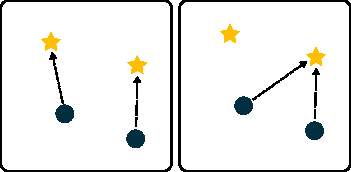
\includegraphics[width=0.7\linewidth]{figures/behavior.pdf}
  \caption{Examples of cooperative and uncoordinated behavior. (Left) desired, agents effectively choose different paths to collect different items. (Right) undesired, agents cover the same path to collect the same item.}
  \label{fig:behavior}
\end{figure}


\subsection{Results}\label{sec:results}

\paragraph{Performance comparison}
The results -- \Cref{fig:results} -- shows that employing a centralized training (i.e., CTDE) approach allows the model to converge 
 more rapidly -- in terms of episodes -- to a higher reward compared to a fully decentralized approach (i.e., DTDE). 
%
This difference becomes even more evident when considering the Mean Episode Length metric, where CTDE not only converges 
 faster but also solves the task using shorter episodes than DTDE. 
 
Additionally, we implemented another state-of-the-art algorithm, namely MAPPO, as a baseline for comparison. 
%
However, MAPPO performed worse than both CTDE and DTDE across both metrics -- yielding lower results and exhibiting less stability, 
 as reflected in its higher standard deviation.

Regarding the proposed neighbor-based approaches, it can be observed that both \emph{experience sharing} and 
 \emph{NN averaging} enhance the performance of DTDE, achieving results comparable to CTDE while also increasing 
 learning stability. 
% 
On the other hand, \emph{NN consensus} maintains performance levels similar to DTDE, which may be attributed to the 
 simplicity of the implemented consensus policy. 
%
Nevertheless, it remains more stable and achieves better performance than MAPPO.

\paragraph{Scalability}
To evaluate the scalability of the learned policies, we conducted several experiments by increasing the number 
 of agents -- specifically to 8, 16, and 32 -- and measuring the time required to complete the task 
 (i.e., mean episode length). 

The results -- \Cref{fig:time-eval} -- show that as the number of agents increases, DTDE exhibits both a higher mean time 
 to solve the task and greater instability. 
%
In contrast, CTDE, NN averaging, and experience sharing maintain strong performance. 
%
Similar to the training phase, NN consensus does not achieve the same results as the other two neighbor-based 
 approaches but remains on par with DTDE in terms of performance.


\paragraph{Communication overhead}

The proposed neighbor-based approaches, particularly NN averaging and experience sharing, achieve performance
 comparable to CTDE while maintaining a decentralized learning structure similar to DTDE. 
% 
However, this entails a communication overhead due to the information agents must exchange with their neighbors
 -- see \Cref{fig:scalability}. 
%
For NN consensus, the overhead remains constant, as each agent selects the best neighbor and only exchanges 
 information with that agent, meaning the amount of data shared does not increase with the number of neighbors. 
% 
In contrast, for NN averaging and experience sharing, the overhead scales linearly. 
%
Specifically, the growth in overhead for experience sharing is minimal, as the agents' experiences require very 
 little memory. 
%
For NN averaging, however, this increase is more significant, as even a moderately complex neural network 
 has a substantially larger memory footprint.
% 
Nevertheless, for all approaches, the overhead remains within a few megabytes (less than 25MB) when dealing with 
 up to 10 neighboring agents.
%
This makes all approaches feasible, although in scenarios with limited communication resources, experience 
 sharing would be the optimal choice, as it provides performance similar to NN averaging but with 
 much lower overhead.


% \begin{itemize}
% \item \textbf{Performance comparison:}
% \begin{itemize}
% \item Present the results of each distributed strategy against the centralized training baseline.
% \item Use graphs and statistical analysis to compare the average episode length and average reward.
% \item Highlight which neighbor-based methods perform comparably to centralized training.
% \end{itemize}
% \item \textbf{Scalability analysis:}
% \begin{itemize}
% \item Describe how the experiments were modified to assess scalability (increasing agents, spawn area).
% \item Show how each method scales with the increasing complexity, using appropriate visualizations.
% \item Discuss the implications of using pre-trained models with a larger number of agents.
% \end{itemize}
% \item \textbf{Communication overhead analysis:}
% \begin{itemize}
% \item Quantify the amount of information exchange for each strategy.
% \item Compare the communication overhead across different neighborhood sizes, possibly using graphs.
% \item Discuss the trade-offs between performance and communication efficiency.
% \item Mention potential techniques for reducing communication overhead.
% \end{itemize}
% \end{itemize}

\begin{figure}
  \centering
  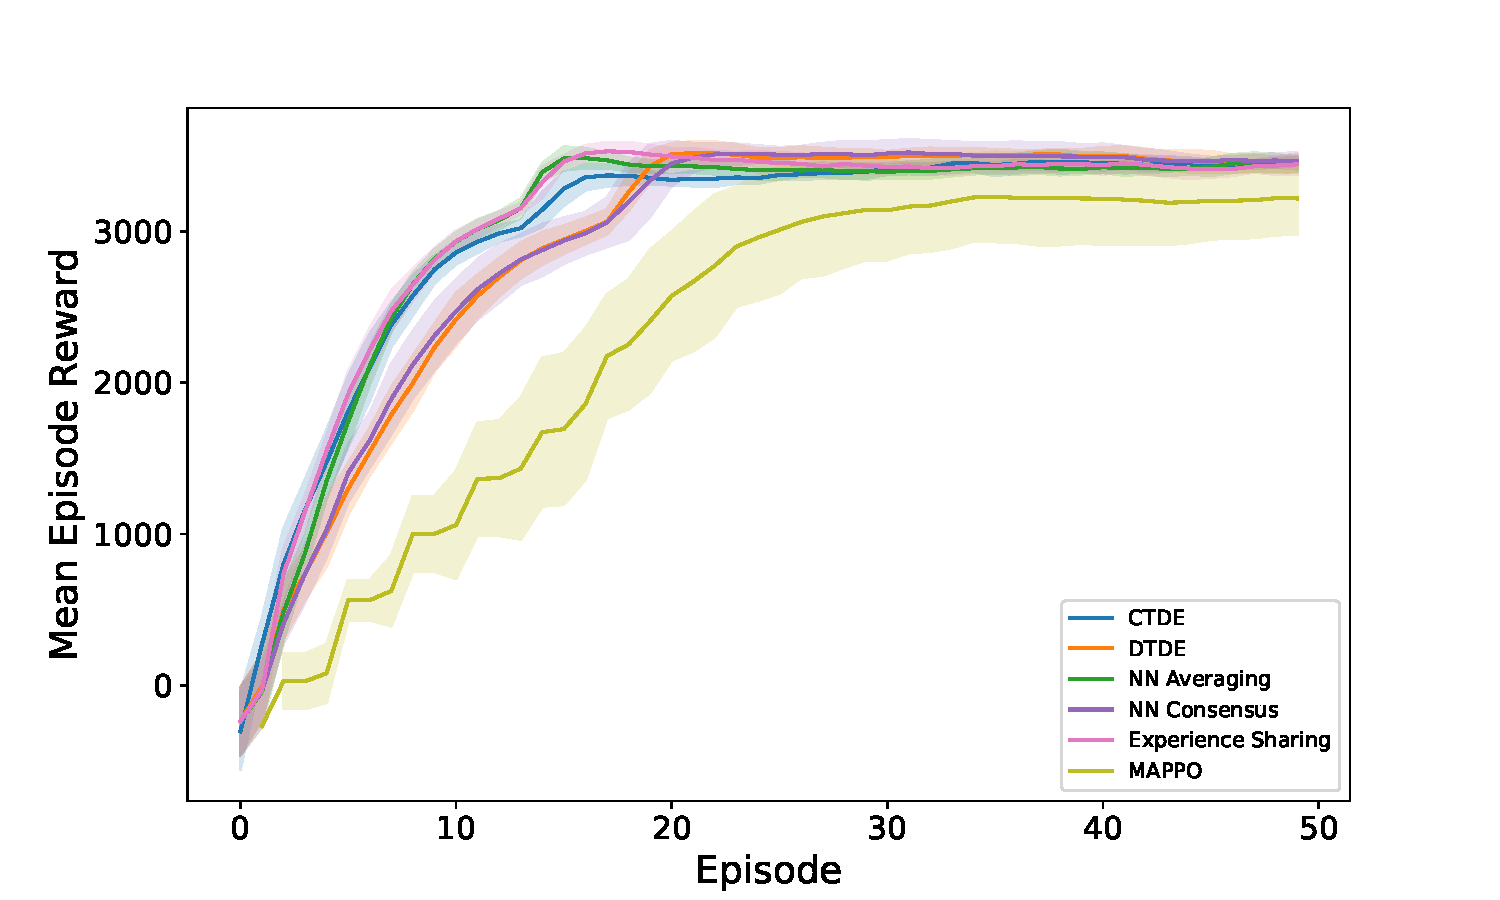
\includegraphics[width=1\linewidth]{figures/episode_reward_mean.pdf}
  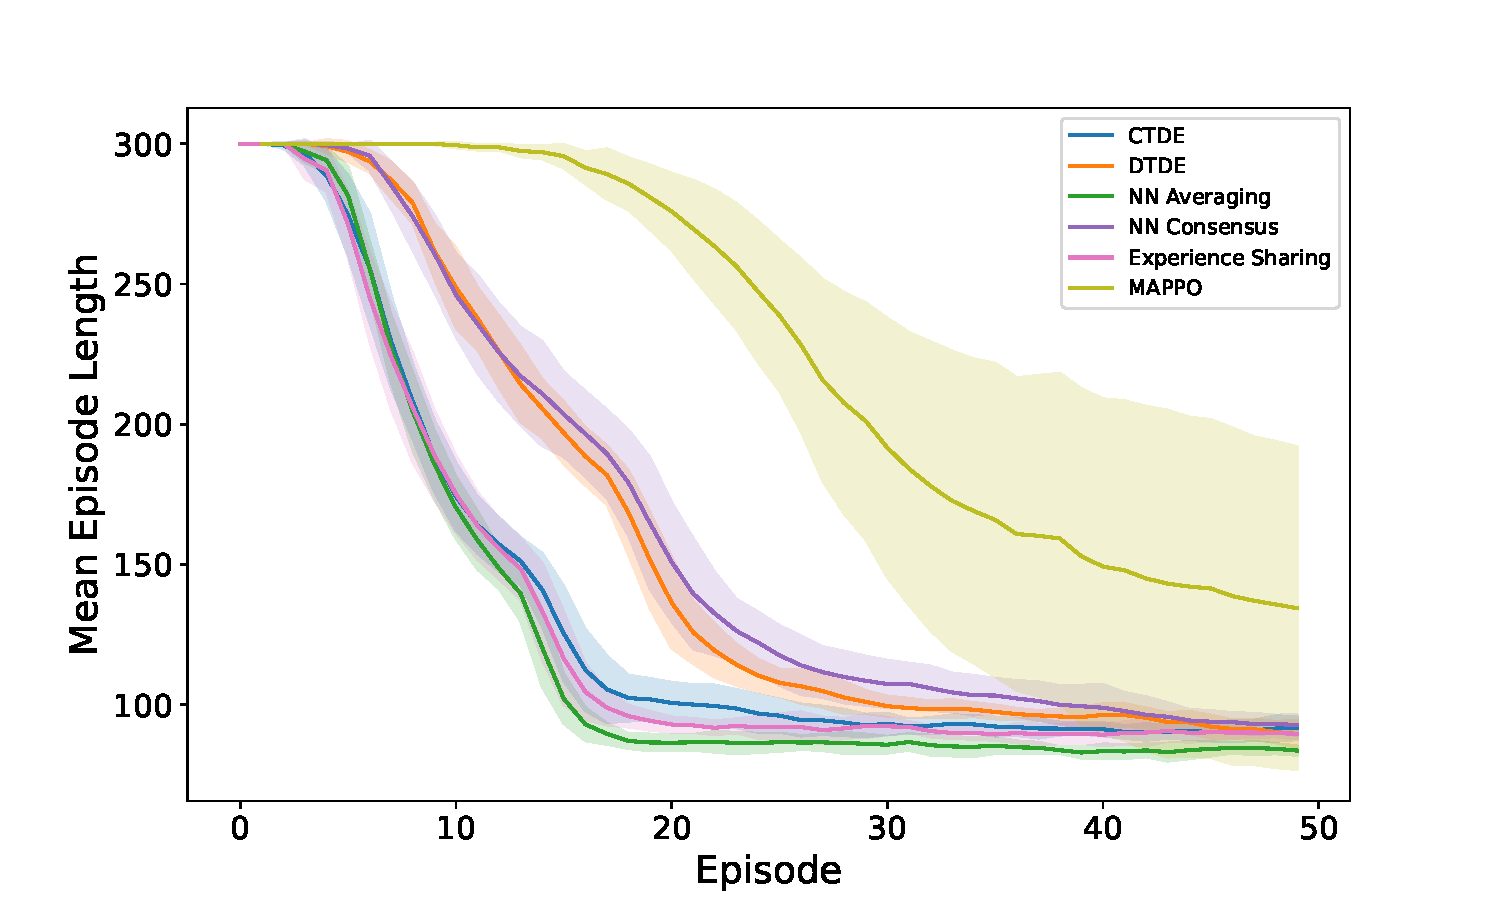
\includegraphics[width=1\linewidth]{figures/episode_len_mean.pdf}
  \caption{Data collected during training. 
  We can see that two of the three neighbor-based strategies achieve performance similar to CTDE.
  }
  \label{fig:results}
\end{figure}

\begin{figure*}[htb]
  \centering
  \begin{subfigure}[b]{0.3\textwidth}
      \centering
      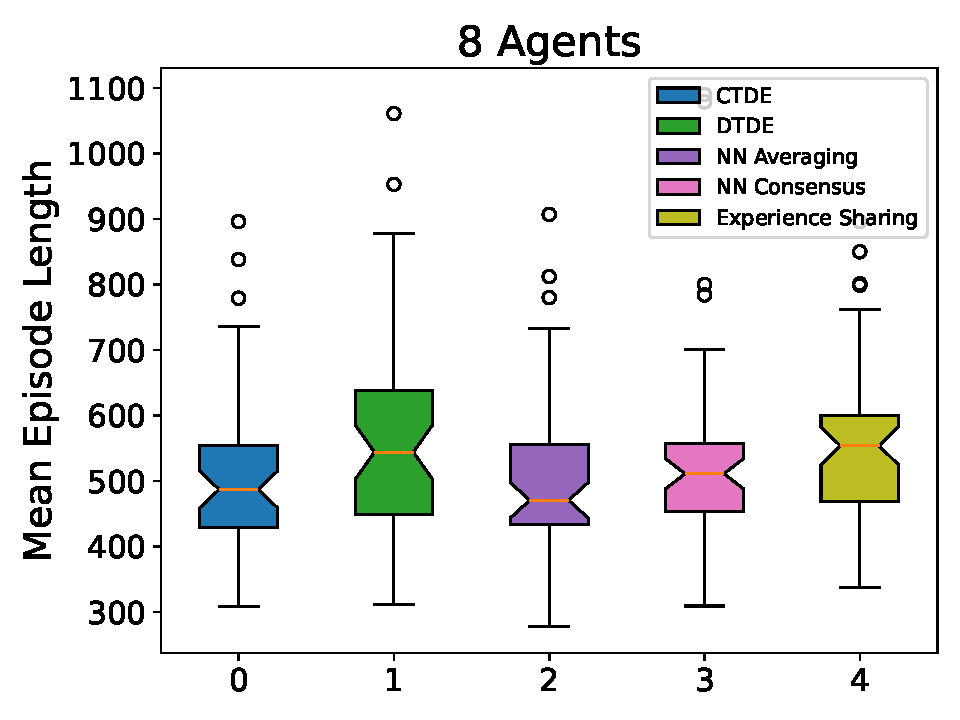
\includegraphics[width=\textwidth]{figures/mean-time-comparison-8-agents.pdf}
      %\caption{Start of the simulation.}
      % \label{fig:zones1}
  \end{subfigure}
  \begin{subfigure}[b]{0.3\textwidth}
      \centering
      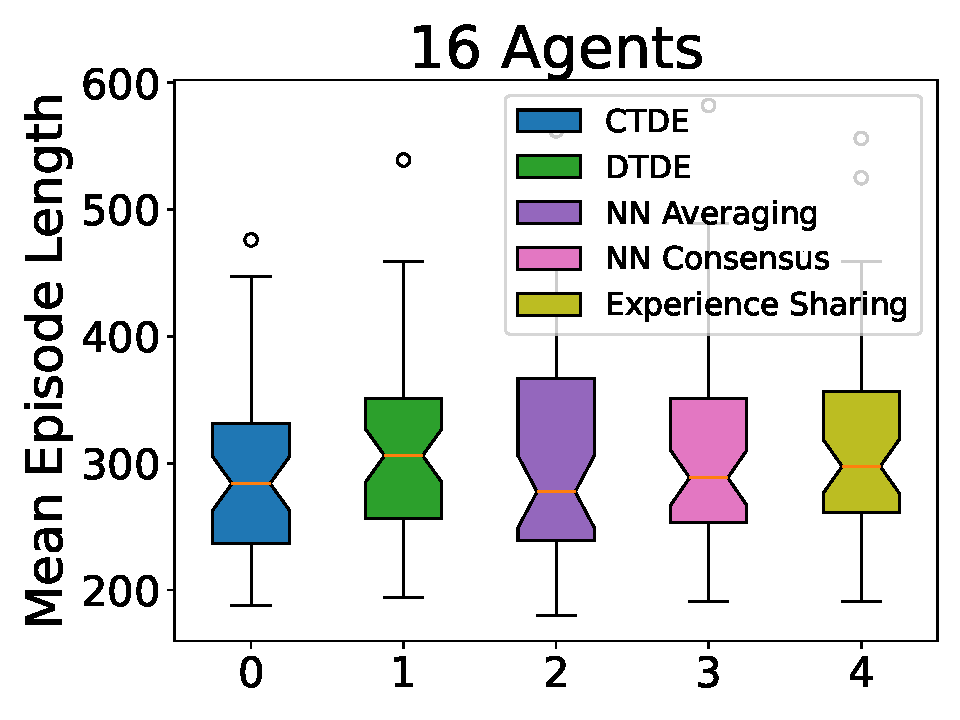
\includegraphics[width=\textwidth]{figures/mean-time-comparison-16-agents.pdf}
      %\caption{After k time steps of the simulation.}
      % \label{fig:zones2}
  \end{subfigure}
  \begin{subfigure}[b]{0.3\textwidth}
      \centering
      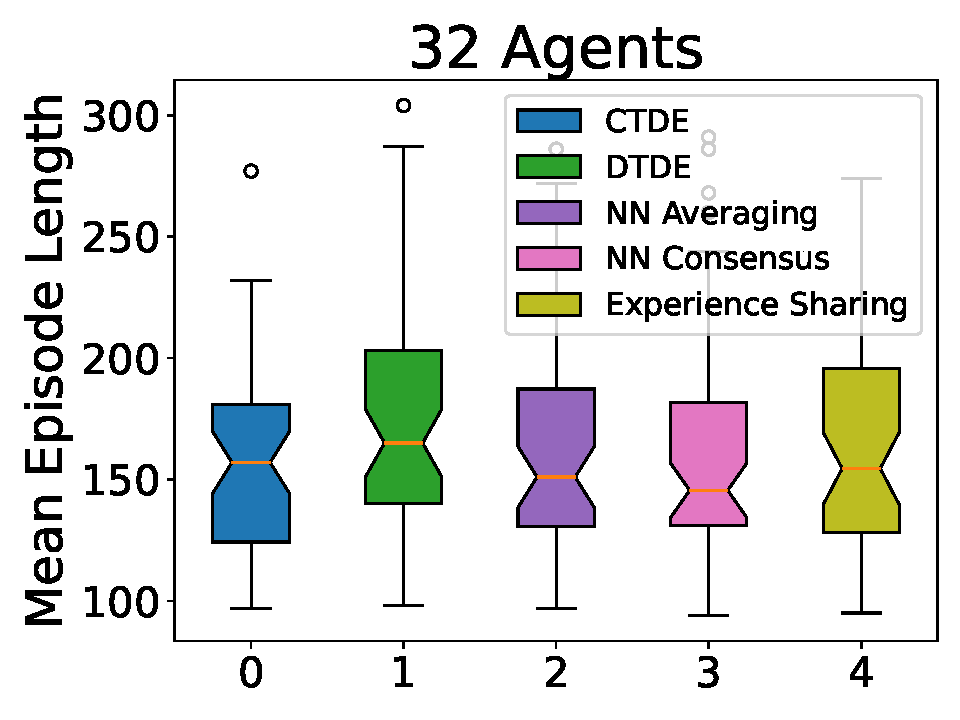
\includegraphics[width=\textwidth]{figures/mean-time-comparison-32-agents.pdf}
      %\caption{End of the simulation.}
      % \label{fig:zones3}
  \end{subfigure}
  \caption{ Data collected during evaluation.
  We can see how, increasing the number of agents, the DTDE methods become more unstable and takes more 
  steps to solve the task, while neighbor-based strategies maintain -- on average -- results comparable to CTDE.
  }
  \label{fig:time-eval}
\end{figure*}

\begin{figure}
  \centering
  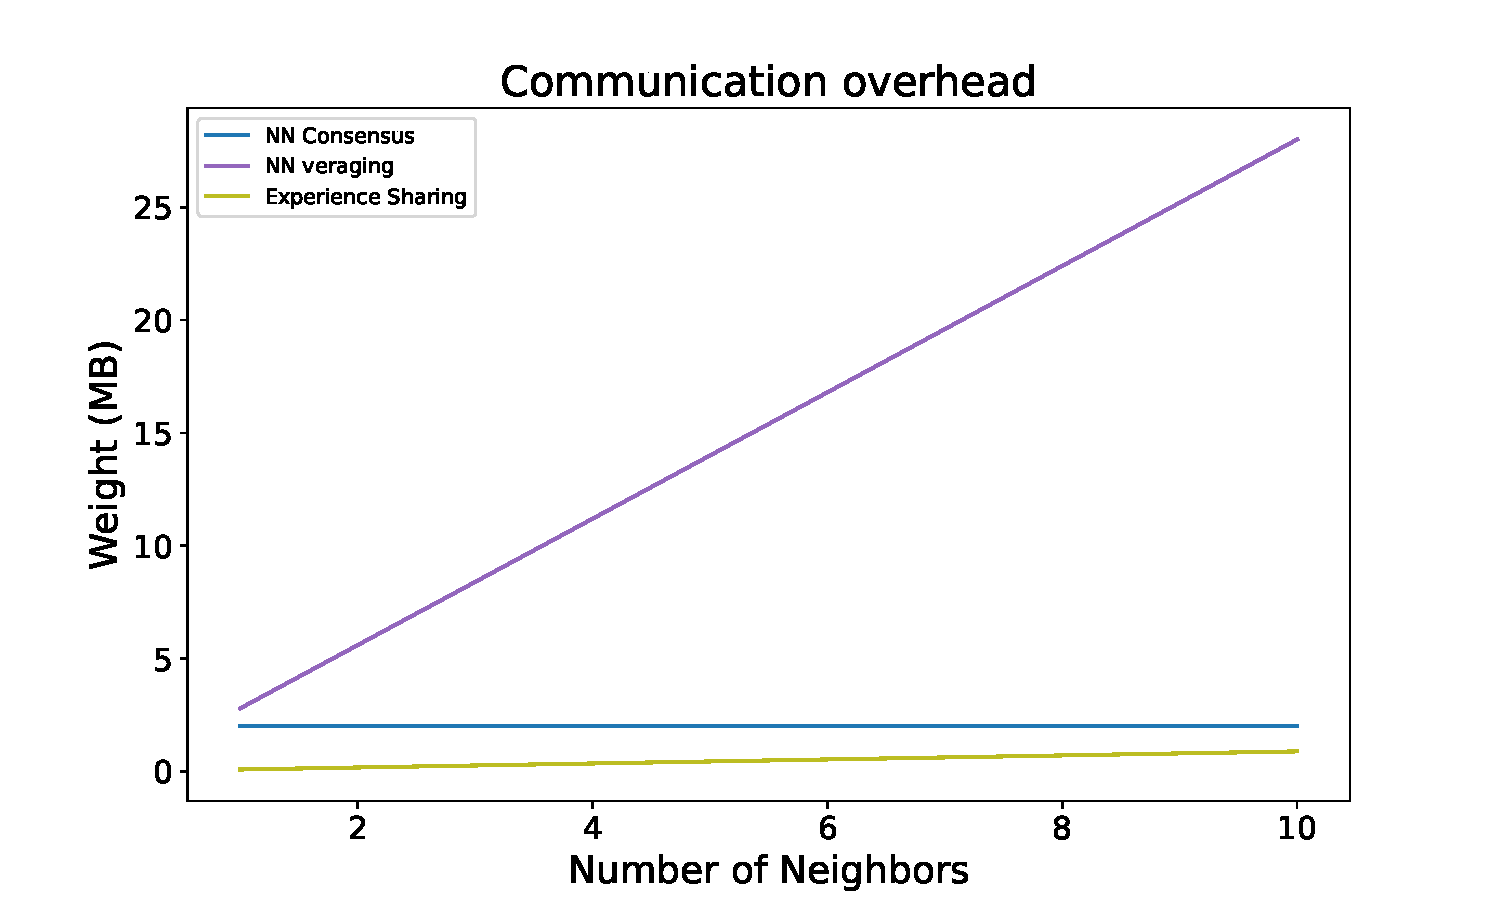
\includegraphics[width=1\linewidth]{figures/scalability.pdf}
  \caption{ Communication overhead due to different neighboring strategies.
  }
  \label{fig:scalability}
\end{figure}


\section{Conclusion}\label{sec:conclusion}
This paper proposes several neighbor-based strategies to achieve decentralized multi-agent learning (i.e., DTDE )with performance 
 comparable to centralized approaches (i.e., CTDE). 
%
These strategies offer the flexibility of DTDE while retaining the stability and performance of CTDE. 
%
Specifically, we introduce three approaches, namely: NN Averaging, NN Consensus and Experience Sharing
 which have been evaluated against various baselines, including CTDE, DTDE based on DQN, and MAPPO. 
%
The results show that two of the three proposed methods significantly enhance DTDE performance, achieving outcomes comparable 
 to CTDE, while NN consensus falls short of this goal, maintaining performance similar to DTDE. 
%
Furthermore, we analyzed the communication overhead, demonstrating that it remains minimal across all cases, 
 particularly with experience sharing, making it suitable for scenarios with very limited communication resources.

Future works may include several promising directions, namely:
\begin{enumerate*}[label=(\roman*)]
  \item explore the implementation of more advanced consensus algorithms to determine if this strategy can also achieve 
   results comparable to the other two;
  \item develop more sophisticated communication protocols to further reduce communication overhead; and
  \item test these approaches in a wider range of, and more complex, scenarios than the one considered in this paper.
\end{enumerate*} 


\bibliographystyle{ACM-Reference-Format}
\bibliography{bibliography} 

\end{document}
